\documentclass{article}

\usepackage[preprint]{neurips_2024}

\usepackage[utf8]{inputenc}
\usepackage[T1]{fontenc}
\usepackage{hyperref}
\usepackage{url}
\usepackage{booktabs}
\usepackage{amsfonts}
\usepackage{amsmath}
\usepackage{graphicx}
\usepackage{microtype}
\usepackage{xcolor}
\usepackage{multirow}

\title{Predicting Short-Term Stock Market Volatility Using Time Series and Machine Learning Models}

\author{%
  Mehul Khajuria \\
  Section ID: 8 \\
  NetID: mk2147 \\
  Department of Computer Science \\
  Rutgers University--New Brunswick
}

\begin{document}

\maketitle

\begin{abstract}
This project studies whether historical price and volume data can forecast short-term equity-market volatility in a leakage-safe setting. I build a reproducible Python pipeline around daily Yahoo Finance OHLCV data for SPY and seven large-cap technology stocks from 2014-01-01 through the most recent available trading date in the local run, 2026-04-24. The primary target is future 5-day realized volatility for SPY. The pipeline constructs log returns, rolling realized volatility, lagged returns and volatility, rolling volume features, RSI, Bollinger Band features, MACD features, and cross-symbol volatility context. I compare naive persistence, rolling-mean persistence, GARCH(1,1), Random Forest, XGBoost gradient boosting, and an MLP neural fallback model after TensorFlow and PyTorch were unavailable in the Python 3.13 environment. On the held-out 2023-01-03 through 2026-04-24 test period, XGBoost achieved the lowest RMSE (0.0839 annualized volatility), followed by Random Forest (0.0875) and the rolling-mean baseline (0.0899). The results suggest that tree-based tabular models can modestly improve point forecasts over simple baselines, but the strong rolling baseline and uneven GARCH/neural-fallback results emphasize the difficulty of stable volatility forecasting. Code: \url{https://github.com/mehulkhajuria/stock-volatility-forecasting-final} Video: \url{TODO_PUBLIC_VIDEO_URL}
\end{abstract}

\section{Introduction}
Financial prices are difficult to predict, but volatility is often more forecastable than the direction of returns. Volatility clustering means that large moves tend to be followed by large moves and quiet periods tend to persist. This property is important for risk management, options pricing, and portfolio sizing, where the question is not always whether SPY will rise tomorrow, but whether near-term uncertainty is likely to increase.

The research question is: \emph{Can time-series and machine learning models predict short-term SPY realized volatility using only information available at the forecast date?} I focus on SPY because it is liquid, broad, and widely used as a market benchmark. Additional symbols, AAPL, MSFT, NVDA, GOOGL, AMZN, TSLA, and META, are used as contextual market features and for volatility correlation analysis. The goal is deliberately narrow: compare forecasting approaches for SPY volatility rather than turn the project into a broad stock-picking system.

The main contribution is a complete reproducible data science pipeline. Although the raw OHLCV data are publicly available through Yahoo Finance, the processed volatility forecasting dataset, engineered features, model comparison pipeline, and evaluation analysis were created specifically for this project. The paper reports only metrics and plots produced by the code in this repository.

\section{Related Work}
Classical time-series forecasting is often framed through autoregressive and moving-average structure \citep{box2015time}. For financial volatility, ARCH and GARCH models are standard baselines because they model conditional variance directly and encode volatility clustering \citep{engle1982arch,bollerslev1986garch}. Realized volatility forecasting extends this idea by using empirical variation in high-frequency or daily returns as the quantity to forecast \citep{andersen2003realized}.

Machine learning methods offer a different route. Random Forests average many decorrelated trees and can capture nonlinear relationships with limited preprocessing \citep{breiman2001random}. Gradient boosting, especially XGBoost, builds trees sequentially to correct earlier residuals and often performs strongly on structured tabular data \citep{chen2016xgboost}. Recurrent neural networks such as LSTMs were designed to model sequential dependence \citep{hochreiter1997lstm}, but in small financial datasets they can be sensitive to implementation details, training length, and regime shifts.

Evaluation protocol matters as much as model choice. Random shuffling can leak future market regimes into training and validation. For that reason, the project uses chronological splits and evaluates only on dates after the training and validation windows, following the spirit of time-series evaluation cautions in \citet{bergmeir2018note}. Pairwise forecast differences are summarized with a Diebold-Mariano style paired loss test \citep{diebold1995comparing}.

\section{Data and Preprocessing}
Daily OHLCV data are downloaded through \texttt{yfinance} \citep{yfinance}. The run used in this paper downloaded data from 2014-01-01 through 2026-04-24. After feature construction and missing-value removal, the SPY modeling table contains 3,061 rows: 1,980 training rows, 251 validation rows, and 830 final test rows. The chronological split is:
\begin{itemize}
  \item train: 2014-01-01 through 2021-12-31,
  \item validation: 2022-01-01 through 2022-12-31,
  \item test: 2023-01-01 through the most recent available date.
\end{itemize}

Adjusted close prices are used for returns. For each symbol, log returns are
\[
r_t=\log(P_t/P_{t-1}).
\]
Annualized realized volatility is computed as a rolling standard deviation of log returns multiplied by $\sqrt{252}$ for 5, 10, and 20 trading-day windows. The prediction target is future 5-day realized volatility:
\[
y_t = RV^{(5)}_{t+5}.
\]
Because $RV^{(5)}_{t+5}$ is the rolling standard deviation ending at $t+5$, it uses returns from $t+1$ through $t+5$. Features at row $t$ use only data available at or before $t$. This target construction is the central leakage-prevention rule in the project code.

Feature engineering includes lagged returns up to 30 days, lagged 5-day volatility up to 30 days, rolling volume means and ratios, RSI, Bollinger Band width and percent-b, MACD, MACD signal, MACD histogram, and same-day 5-day realized volatility context from the seven comparison symbols. Figure~\ref{fig:vol} shows SPY realized volatility over the sample and Figure~\ref{fig:corr} shows that large-cap volatility is highly correlated across symbols, which supports using cross-symbol volatility as context while keeping SPY as the target.

\begin{figure}[t]
  \centering
  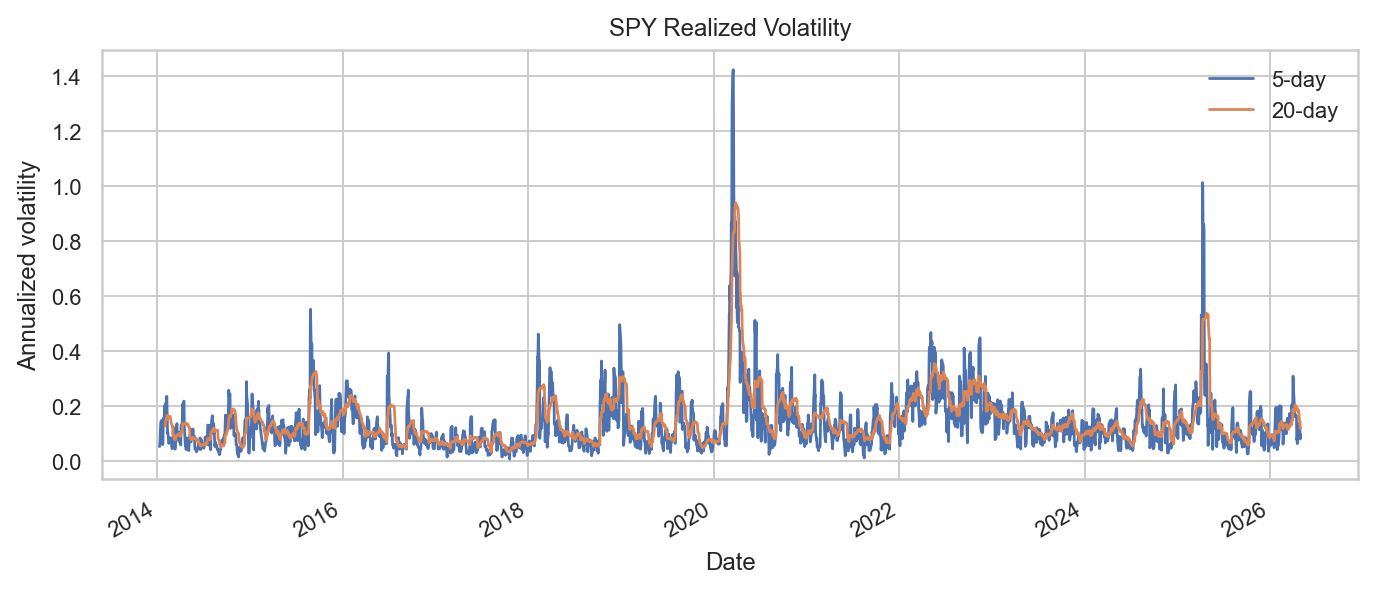
\includegraphics[width=0.9\linewidth]{figures/volatility_timeseries.png}
  \caption{SPY 5-day and 20-day realized volatility. The series shows persistent volatility regimes and abrupt spikes.}
  \label{fig:vol}
\end{figure}

\begin{figure}[t]
  \centering
  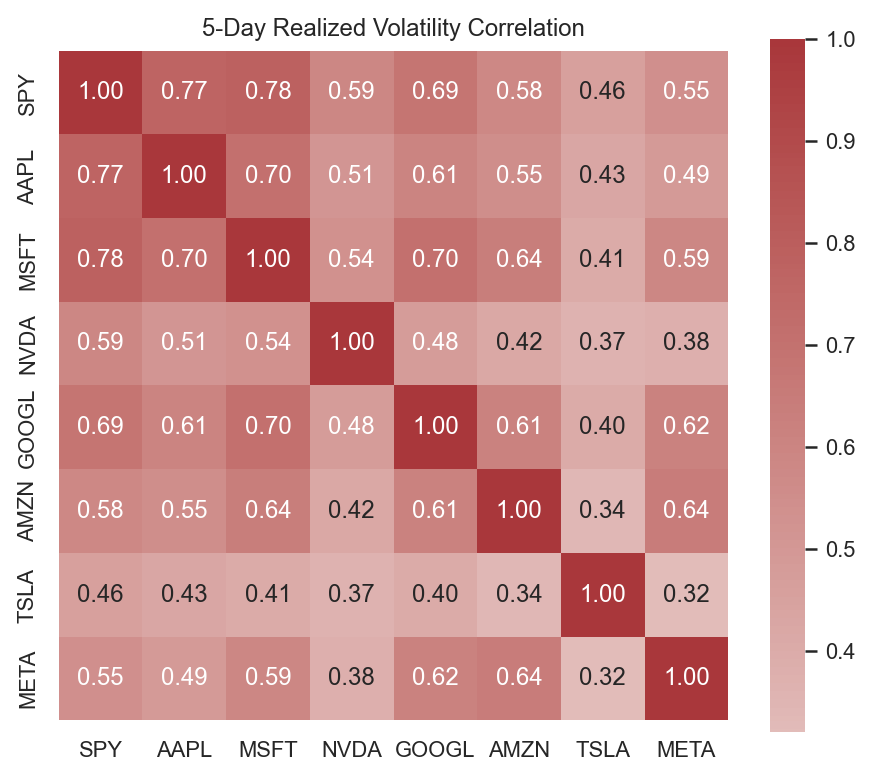
\includegraphics[width=0.62\linewidth]{figures/volatility_correlation_heatmap.png}
  \caption{Correlation heatmap for 5-day realized volatility across SPY and comparison equities.}
  \label{fig:corr}
\end{figure}

\section{Method}
The project compares six forecasting approaches. Naive persistence predicts that future volatility equals current 5-day realized volatility. The rolling-mean baseline predicts with the mean of the previous 20 volatility lags. GARCH(1,1) is fit on train-plus-validation SPY percentage log returns with a constant mean and normal innovations; its multi-step variance forecast is annualized to match the target scale.

The Random Forest model uses 300 trees, maximum depth 10, minimum leaf size 5, and a deterministic random seed. Gradient boosting uses XGBoost with 300 trees, depth 3, learning rate 0.03, row subsampling 0.85, and column subsampling 0.85. These parameters are intentionally conservative because the final test period is held out and not used for iterative tuning. For the neural model, the code first attempts a TensorFlow/Keras LSTM and then a PyTorch LSTM. In this environment neither package was installed for Python 3.13, so the reported neural row is a deterministic scikit-learn MLP fallback. The paper therefore does not claim an LSTM result; it documents the attempt and limitation.

\section{Experimental Setup}
All models are evaluated on the same held-out SPY test period. The primary point-forecast metrics are MSE, MAE, and RMSE. Directional accuracy measures whether a model correctly predicts whether future volatility rises or falls relative to current 5-day volatility:
\[
\mathbb{1}\left[\mathrm{sign}(\hat{y}_t - RV^{(5)}_t)=\mathrm{sign}(y_t - RV^{(5)}_t)\right].
\]
This is useful because volatility management may care about the direction of risk even when point errors are imperfect. The naive persistence baseline predicts exactly no change for every row, so directional accuracy is not meaningful for that model and is reported as NA. It remains a valid point-forecast baseline but is not designed for directional movement.

Approximate runtime is measured inside the Python pipeline for each model. Pairwise Diebold-Mariano tests are computed using squared-error loss differences. These tests are approximate because the implementation uses a compact paired loss-difference statistic without a full Newey-West long-run variance adjustment, so they are treated as supporting evidence rather than the sole basis for conclusions.

\section{Evaluation}
Table~\ref{tab:metrics} reports the held-out results. XGBoost gradient boosting is the best model by RMSE, with 0.0839 annualized volatility. Random Forest is second at 0.0875. The rolling-mean baseline is close at 0.0899 RMSE and has the best MAE and best defined directional accuracy, which is an important caution: simple volatility persistence remains a very strong baseline.

\begin{table}[t]
  \centering
  \caption{Held-out SPY test performance, 2023-01-03 through 2026-04-24. Lower MSE, MAE, and RMSE are better.}
  \label{tab:metrics}
  \begin{tabular}{lrrrrr}
    \toprule
    Model & MSE & MAE & RMSE & Dir. Acc. & Seconds \\
    \midrule
    Gradient Boosting & 0.0070 & 0.0583 & 0.0839 & 0.6687 & 0.73 \\
    Random Forest & 0.0077 & 0.0587 & 0.0875 & 0.6518 & 24.19 \\
    Rolling Mean & 0.0081 & 0.0525 & 0.0899 & 0.6892 & 0.00 \\
    Naive Persistence & 0.0088 & 0.0582 & 0.0941 & NA & 0.00 \\
    GARCH(1,1) & 0.0145 & 0.0999 & 0.1204 & 0.5530 & 0.05 \\
    MLP neural fallback & 0.0165 & 0.0931 & 0.1286 & 0.5952 & 0.49 \\
    \bottomrule
  \end{tabular}
\end{table}

The model comparison plot in Figure~\ref{fig:comparison} makes the ranking visible. Figure~\ref{fig:pred} overlays actual volatility against the best model. The boosted model follows broad regimes, but like most daily volatility models it smooths the sharpest changes. Figure~\ref{fig:error} shows forecast-error distributions. The boosted and forest models are centered closer to zero than GARCH and the neural fallback, but all models retain sizable tails.

\begin{figure}[t]
  \centering
  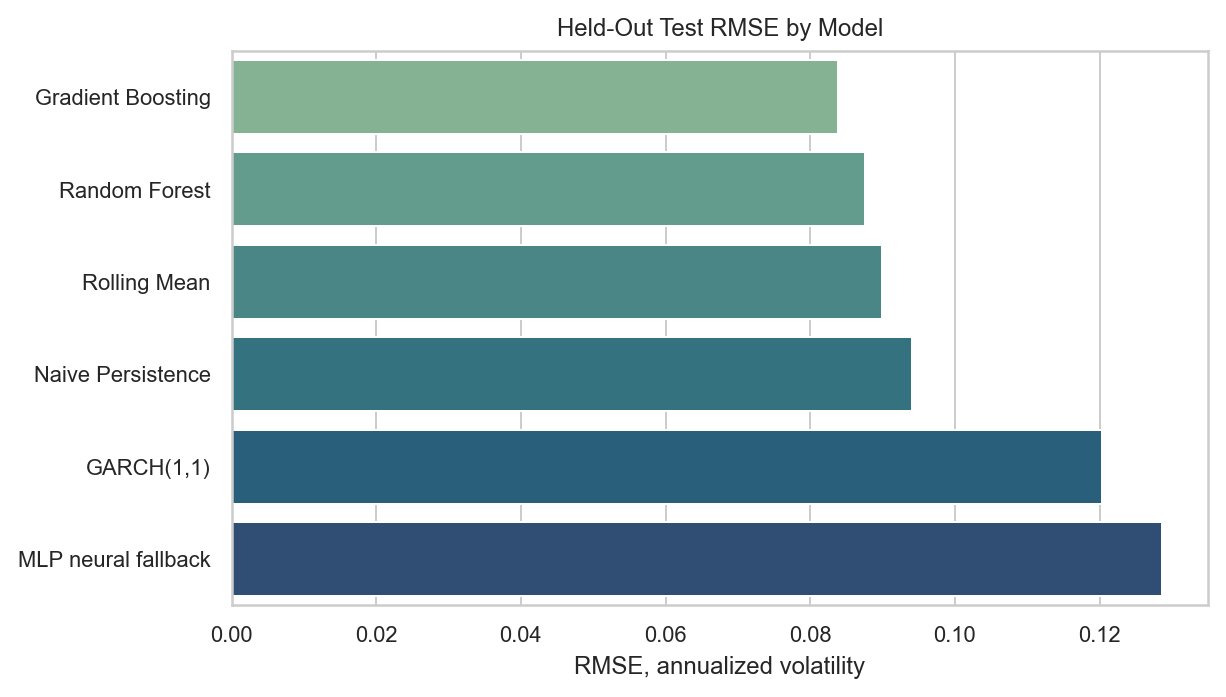
\includegraphics[width=0.76\linewidth]{figures/model_comparison.png}
  \caption{Held-out test RMSE by model.}
  \label{fig:comparison}
\end{figure}

\begin{figure}[t]
  \centering
  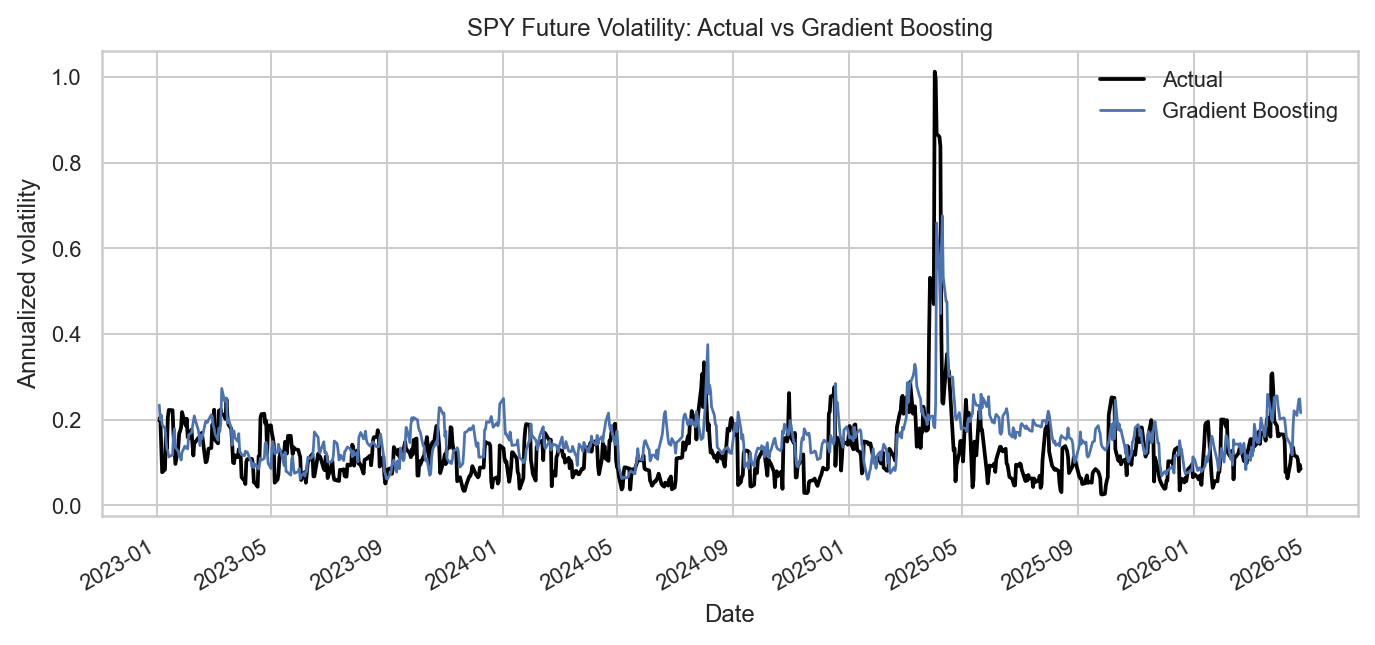
\includegraphics[width=0.9\linewidth]{figures/predicted_vs_actual.png}
  \caption{Actual future 5-day realized volatility versus the best RMSE model.}
  \label{fig:pred}
\end{figure}

\begin{figure}[t]
  \centering
  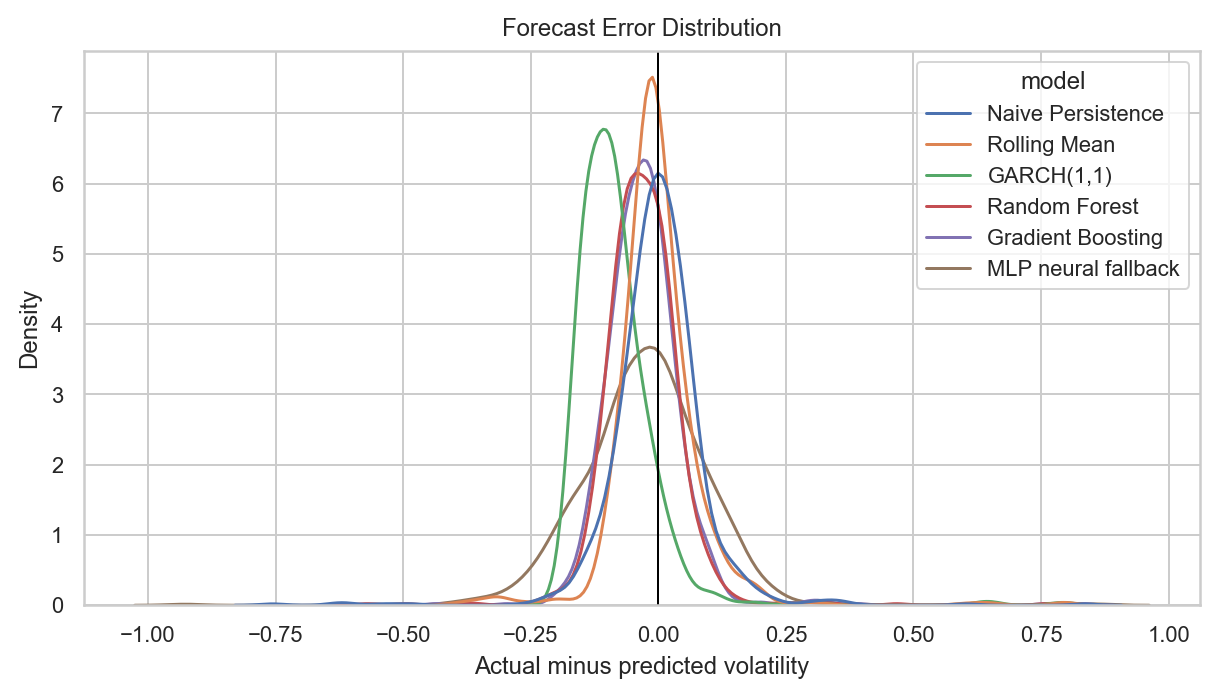
\includegraphics[width=0.82\linewidth]{figures/error_distribution.png}
  \caption{Held-out forecast error distributions, actual minus predicted volatility.}
  \label{fig:error}
\end{figure}

Pairwise Diebold-Mariano tests support the broad ranking. For example, Gradient Boosting has lower squared-error loss than GARCH with $p=1.15\times 10^{-21}$, and lower loss than the neural fallback with $p=6.73\times 10^{-15}$. Random Forest also beats GARCH with $p=2.02\times 10^{-14}$. The rolling mean beats GARCH strongly, but its comparison with the two tree models is closer, which again shows that the practical improvement over simple persistence is modest.

\begin{table}[t]
  \centering
  \caption{Selected pairwise Diebold-Mariano style comparisons using squared-error loss. Negative statistics mean model A has lower average loss than model B.}
  \label{tab:dm}
  \begin{tabular}{llrr}
    \toprule
    Model A & Model B & DM stat. & $p$-value \\
    \midrule
    Rolling Mean & GARCH(1,1) & -11.06 & $1.29\times 10^{-26}$ \\
    GARCH(1,1) & Gradient Boosting & 9.84 & $1.15\times 10^{-21}$ \\
    Gradient Boosting & MLP neural fallback & -7.12 & $2.35\times 10^{-12}$ \\
    GARCH(1,1) & Random Forest & 7.79 & $2.02\times 10^{-14}$ \\
    Random Forest & MLP neural fallback & -6.93 & $8.48\times 10^{-12}$ \\
    Rolling Mean & MLP neural fallback & -5.69 & $1.73\times 10^{-8}$ \\
    \bottomrule
  \end{tabular}
\end{table}

\subsection{Regime-Based Error Analysis}
Aggregate RMSE can hide where models succeed or fail. To check this, I split the held-out test observations into low-volatility, middle-volatility, and high-volatility regimes using the 25th and 75th percentiles of the actual future-volatility target. In the test set, these thresholds are 0.0792 and 0.1508 annualized volatility, respectively. This diagnostic is not used for training; it is an after-the-fact error analysis of the same held-out predictions.

\begin{table}[t]
  \centering
  \caption{RMSE by held-out volatility regime. Low and high regimes are the bottom and top quartiles of actual future volatility.}
  \label{tab:regime}
  \begin{tabular}{lrrr}
    \toprule
    Model & Low vol. & Middle vol. & High vol. \\
    \midrule
    Gradient Boosting & 0.0902 & 0.0543 & 0.1187 \\
    Random Forest & 0.0858 & 0.0546 & 0.1315 \\
    Rolling Mean & 0.0656 & 0.0585 & 0.1453 \\
    Naive Persistence & 0.0694 & 0.0546 & 0.1567 \\
    GARCH(1,1) & 0.1529 & 0.0984 & 0.1232 \\
    MLP neural fallback & 0.1243 & 0.1020 & 0.1727 \\
    \bottomrule
  \end{tabular}
\end{table}

This split explains why the overall ranking is nuanced. In low-volatility periods, the rolling mean and naive persistence baselines perform best. Their bias toward recent calm conditions is useful when markets remain calm. In high-volatility periods, however, Gradient Boosting has the best RMSE, followed closely by GARCH. The tree model appears better at using the wider feature set to respond when volatility is elevated, while simple persistence lags sharp transitions. The middle-volatility regime is where the models are closest: Gradient Boosting, Naive Persistence, and Random Forest all sit near 0.054 RMSE. These diagnostics make the headline result more cautious. The boosted model wins overall, but its advantage is concentrated in harder, higher-volatility periods rather than uniformly dominating every market state.

\subsection{What the Figures Add}
The six generated figures are included because each answers a different audit question. The volatility time series verifies that the target has meaningful temporal structure and captures major market regimes. The correlation heatmap verifies that the comparison symbols provide related market context rather than unrelated noise. The predicted-versus-actual plot checks whether the best model follows the level of volatility through time, not only whether it has a good scalar score. The model comparison plot makes the RMSE ranking transparent. The error distribution plot checks for skewness and heavy tails. The feature-importance plot checks whether the tree model relies on plausible, time-available predictors. Together these figures help guard against a common failure mode in machine learning projects: reporting a table of metrics without explaining whether the dataset, target, plots, and model behavior agree.

\section{Discussion}
The strongest result is not that one model ``solves'' volatility forecasting. Instead, the results show a layered pattern. First, volatility persistence is powerful: the rolling mean baseline is competitive with machine learning and has the highest directional accuracy. Second, tree-based models can improve RMSE by combining current volatility, longer volatility windows, lagged volatility, market context, and technical indicators. Third, GARCH underperforms in this run, likely because the implementation is fit once on the pre-test period and forecasts many steps ahead, while the test target is realized 5-day volatility rather than one-day conditional variance.

Feature importance in Figure~\ref{fig:importance} is consistent with financial intuition. Current 5-day realized volatility, 20-day realized volatility, and the first lag of volatility dominate. Bollinger positioning, MSFT volatility context, MACD terms, volume ratio, and RSI contribute but are secondary. This makes the model interpretable: it is not discovering a mysterious price-direction signal; it is mostly learning persistence and regime context.

\begin{figure}[t]
  \centering
  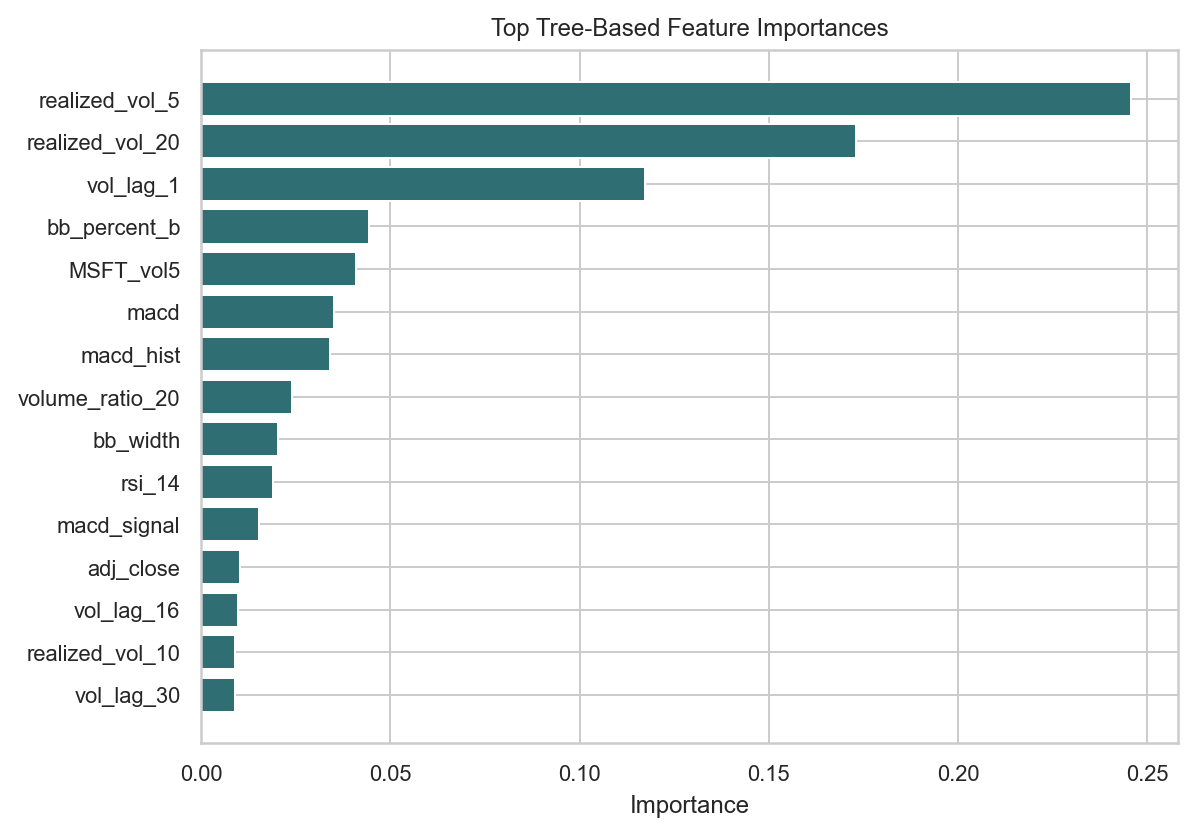
\includegraphics[width=0.78\linewidth]{figures/feature_importance.png}
  \caption{Top Random Forest feature importances.}
  \label{fig:importance}
\end{figure}

\begin{table}[t]
  \centering
  \caption{Top Random Forest feature importances saved by the pipeline.}
  \label{tab:features}
  \begin{tabular}{lr@{\quad}lr}
    \toprule
    Feature & Importance & Feature & Importance \\
    \midrule
    realized\_vol\_5 & 0.2458 & macd & 0.0352 \\
    realized\_vol\_20 & 0.1731 & macd\_hist & 0.0336 \\
    vol\_lag\_1 & 0.1172 & volume\_ratio\_20 & 0.0250 \\
    bb\_percent\_b & 0.0445 & bb\_width & 0.0202 \\
    MSFT\_vol5 & 0.0409 & rsi\_14 & 0.0186 \\
    \bottomrule
  \end{tabular}
\end{table}

There are two useful implications for practitioners. The first is that the forecast target controls the evaluation story. A one-day conditional variance model and a future 5-day realized volatility target are related but not identical. The GARCH row should therefore be read as a conventional statistical baseline adapted to the target, not as the final word on GARCH-family modeling. The second is that interpretability can be a guardrail against accidental leakage. If the top features had been future-shifted columns or same-window target proxies, that would be suspicious. Instead, the dominant features are current and lagged volatility variables that are allowed by the forecasting setup.

\section{Reproducibility and Audit}
The project is organized so that the complete run can be reproduced with \texttt{python -m src.run\_all}. The command downloads or loads cached Yahoo Finance CSV files, builds the processed SPY feature table, trains all available models, computes metrics, writes JSON and CSV summaries, and regenerates all figures. Results are saved in \texttt{results/}, while figures are saved in both \texttt{figures/} and \texttt{paper/figures/}. The generated contact sheet is a quick visual audit for the six required plots.

Several audit checks were performed after generation. All required result files exist: \texttt{metrics.csv}, \texttt{directional\_accuracy.csv}, \texttt{dm\_test\_results.csv}, and \texttt{summary.json}. The major figures are non-empty PNG files with readable dimensions and nonzero pixel variance. The LaTeX paper compiles against \texttt{neurips\_2024.sty}; \texttt{latexmk} could not be used because MiKTeX reported that Perl was unavailable, so the paper was compiled with the standard \texttt{pdflatex}, \texttt{bibtex}, \texttt{pdflatex}, \texttt{pdflatex} sequence. This is a tooling limitation, not a missing style-file or citation issue.

The repository also includes \texttt{requirements.txt}, a full \texttt{requirements-lock.txt} from \texttt{pip freeze}, and \texttt{environment.yml}. Raw Yahoo Finance CSV caches are ignored by git because they can be regenerated and may become stale. The paper and README retain explicit placeholders for the public GitHub and video URLs until those links are created.

\section{Data Ethics and Use}
The data source is public market data, but that does not make the modeling problem consequence-free. Volatility forecasts can influence financial decisions, and a course project should not be represented as a trading recommendation. For that reason, the repository and paper state that the project is not financial advice. The project also avoids claiming that Yahoo Finance data are original data collection. The original work is the reproducible processing and evaluation pipeline.

There are also reproducibility responsibilities. Financial datasets update as new trading days appear, and vendors can revise historical data after splits, dividends, or corrections. A future rerun may therefore produce slightly different end dates or metrics. The pipeline records the actual test start, test end, row counts, model notes, and generation time in \texttt{results/summary.json}. This makes the final paper traceable to a specific run instead of implying that the numbers are timeless constants.

\section{Future Work}
The most direct extension is a true walk-forward experiment. In that version, tree models and GARCH would be periodically refit as the test window advances, which better approximates deployment. A second extension is to add option-implied volatility, such as VIX or SPY option data, because implied volatility directly summarizes market expectations of future risk. A third extension is to use intraday returns to construct higher-resolution realized volatility targets. This would likely make the target less noisy than daily close-to-close realized volatility, but it would also require more careful data storage and computation.

The deep learning component also deserves a cleaner environment. TensorFlow and PyTorch were not installed here, so the pipeline reports a neural fallback. With a supported Python version and GPU or CPU deep-learning stack, a compact LSTM could be trained and compared honestly. Even then, it should be evaluated against the same rolling baseline and tree models, because this project shows that complexity alone is not a reliable advantage in financial forecasting.

\section{Limitations}
This project uses public daily OHLCV data only. It does not use intraday prices, option-implied volatility, macroeconomic announcements, earnings calendars, or news sentiment. Daily realized volatility is a coarse proxy and can miss intraday risk. The GARCH comparison is useful but not exhaustive; a walk-forward refit or alternative distributions could improve it. The LSTM requirement was attempted in code, but the installed Python 3.13 environment did not include TensorFlow or PyTorch, so the actual reported neural metric is an MLP fallback and should not be interpreted as evidence against LSTMs in general.

There are also modeling limitations. Hyperparameter search is intentionally limited to avoid overfitting the final test period. The Diebold-Mariano test is approximate. The comparison symbols are large technology stocks, so the context features may be less useful for non-technology market regimes. Finally, none of the results should be read as trading advice or a deployable risk system without transaction-cost analysis, stress testing, and live out-of-sample monitoring.

\section{Conclusion}
Using a reproducible Yahoo Finance pipeline, this project compares statistical, baseline, machine learning, and neural-fallback approaches for forecasting short-term SPY realized volatility. On the held-out 2023-2026 test period, XGBoost gradient boosting achieved the best RMSE, Random Forest was close, and a simple rolling-mean baseline remained highly competitive. The main lesson is practical: careful target construction, time-aware validation, and strong baselines matter as much as model complexity. For future work, the most promising extensions are walk-forward GARCH refitting, true LSTM training in a supported environment, intraday realized volatility, and option-implied volatility features such as VIX.

\clearpage
\bibliographystyle{plainnat}
\bibliography{references}

\end{document}
